% !TEX program = xelatex
% 编译：xelatex -interaction=nonstopmode rag_comparison.tex （跑两遍生成目录）
\documentclass[11pt,a4paper,fontset=windows]{ctexart}

\usepackage[margin=2.3cm]{geometry}
\usepackage{booktabs}
\usepackage{graphicx}
\usepackage{float}
\usepackage{array}
\usepackage{longtable}
\usepackage{caption}
\usepackage{amsmath}
\usepackage{amssymb}
\usepackage{xcolor}
\usepackage{enumitem}
\usepackage[colorlinks=true,linkcolor=blue!60!black,urlcolor=blue!60!black]{hyperref}

\definecolor{hl}{RGB}{0,90,160}
\newcommand{\best}[1]{\textbf{\textcolor{hl}{#1}}}
\captionsetup{font=small,labelfont=bf}
\setlist{itemsep=2pt,topsep=2pt}

% 允许少量行距拉伸，消除中英混排长 \texttt 串导致的 overfull
\setlength{\emergencystretch}{3em}
\tolerance=2000
\hbadness=4000

\title{\textbf{简历检索 RAG 多形态对比评测报告}\\[4pt]
\large 5 种 RAG 形态在 100 份中英混合简历集上的离线检索质量基准}
\author{ResumAI-Agent · 离线 RAG 评测 Harness}
\date{\today}

\begin{document}
\maketitle

\begin{abstract}
\noindent 本报告在 100 份真实简历（50 份中文 \texttt{.txt} + 50 份英文 \texttt{.pdf}，覆盖 14 个岗位簇）上，
用 28 条中英双语检索查询，严格对比了 \textbf{BM25 / Dense Embedding / Hybrid(RRF) / Agentic RAG / GraphRAG}
五种检索形态的 Precision@5、Recall@10、MRR、nDCG@10、查询时延与 LLM 成本。
所有指标均为\textbf{真实运行结果}，可一键复现；Agentic 与 GraphRAG 的 LLM 调用经 DeepSeek 真实发生并落盘缓存。
核心结论：在本「技能关键词密集」的简历语料上，\best{BM25 是性价比之王}（nDCG@10=0.940，中位时延 2.2\,ms，零成本）；
\best{Agentic RAG 取得最高检索质量}（nDCG@10=0.949、MRR=0.982），但代价是约 \best{2000$\times$ 的时延}与按次计费的 LLM 成本；
Dense（all-MiniLM-L6-v2）因\textbf{英文中心、对中文简历语义弱}而垫底；GraphRAG 查询期极快但实体抽象\textbf{丢失词频/上下文信号}，
在部分查询上明显劣化。全部 LLM 调用 156 次、总成本仅 \textbf{\$0.06}。
\end{abstract}

\tableofcontents
\vspace{6pt}

% ============================================================
\section{结论先行（TL;DR）}
\label{sec:tldr}

\begin{table}[H]
\centering
\caption{五种 RAG 形态主结果（100 简历 / 28 查询，真实运行）。时延为\textbf{中位}单查询时延；
加粗为该列最优。}
\label{tab:main}
\small
\begin{tabular}{lccccrrr}
\toprule
方法 & P@5 & Recall@10 & MRR & nDCG@10 & 中位时延 & LLM 调用 & 估算成本 \\
\midrule
BM25            & 0.943 & \best{0.865} & 0.958 & 0.940 & \best{2.2\,ms}   & 0   & \$0 \\
Dense (MiniLM)  & 0.807 & 0.725 & 0.887 & 0.799 & 333.4\,ms & 0   & \$0 \\
Hybrid (RRF)    & 0.936 & 0.831 & 0.964 & 0.918 & 464.2\,ms & 0   & \$0 \\
Agentic RAG     & \best{0.957} & \best{0.865} & \best{0.982} & \best{0.949} & 5392\,ms & 56\,(查询期) & \$0.027 \\
GraphRAG        & 0.864 & 0.776 & 0.949 & 0.862 & 30.4\,ms  & 100\,(建图期) & \$0.034 \\
\bottomrule
\end{tabular}
\end{table}

\begin{itemize}
\item \textbf{质量排序}：Agentic $>$ BM25 $>$ Hybrid $>$ GraphRAG $>$ Dense（按 nDCG@10）。
\item \textbf{性价比排序}：BM25 $\gg$ 其它——以 0.2\% 的 nDCG 差距换来 $\sim$2000$\times$ 的时延优势和零成本。
\item \textbf{Agentic 的增益是真实的但很小}（nDCG +0.9\%、MRR +2.4\% 相对 BM25），代价巨大；只在「语义/歧义」查询上增益明显。
\item \textbf{Dense 单路最弱}：英文中心的 MiniLM 对中文简历语义召回差（见 \S\ref{sec:findings}）。
\item \textbf{GraphRAG 没有解决本场景的问题}：二值技能图丢失词频与上下文，在 SRE/可观测性等「术语共享」查询上崩塌（nDCG 低至 0.12）。
\end{itemize}

% ============================================================
\section{评测设计}
\label{sec:design}

\subsection{数据集}
评测语料为仓库内 \texttt{testdata/stress\_resumes/}，共 \textbf{100 份简历} + \texttt{manifest.json}：

\begin{itemize}
\item \textbf{文件形态}：50 份 \texttt{.txt}（真实中文正文）+ 50 份 \texttt{.pdf}（英文/拼音内容）。
      \texttt{.txt} 以 UTF-8 直接读取；\texttt{.pdf} 用 \texttt{PyMuPDF} 抽取文本（平均 614 token/份）。
\item \textbf{岗位簇}：14 个，含资深后端(12)、AI~Agent(10)、大模型应用(8)、产品经理(8)、资深/初级前端(各7)、
      数据平台(7)、运维~SRE(7)、后端(7)、应届后端(6)、算法(6)、测试(5)、安全(5)、Android(5)。
\item \textbf{元数据}：每份含 \texttt{role}（中文岗位）与 \texttt{expectedSkills}（英文技能标签，全集 92 个）。
\item \textbf{中英混排特性}：中文简历正文中\textbf{大量嵌入英文技术词}（如 Spring~Boot、Kafka、Redis、JVM、Prometheus），
      这是 BM25 在本语料强势的根本原因（见 \S\ref{sec:findings}）。
\end{itemize}

\subsection{查询集}
共 \textbf{28 条}查询（落盘 \texttt{queries.json}），覆盖全部 14 个岗位簇及若干跨簇/语义查询。
每条同时给\textbf{中文与英文}版本，检索时拼接二者，以同时适配中文 \texttt{.txt} 与英文 \texttt{.pdf}。
检索器\textbf{只能看到查询文本}，绝不接触 ground-truth 的目标技能，避免数据泄漏。

\begin{table}[H]
\centering
\caption{查询集示例（节选）。}
\label{tab:queries}
\small
\begin{tabular}{llp{4.6cm}p{4.6cm}}
\toprule
ID & 目标簇 & 中文 & English \\
\midrule
q01 & 资深后端 & 高并发后端 Kafka 微服务 可观测性 SLA 治理 & high concurrency backend Kafka microservices observability \\
q05 & AI Agent & RAG 向量检索 Agent 工程 LangGraph 工具编排 & RAG vector retrieval agent engineering LangGraph \\
q13 & 运维/SRE & Kubernetes DevOps SRE 监控 CI/CD 容器化 & Kubernetes DevOps SRE monitoring CI/CD Docker \\
q14 & 算法 & 推荐算法 机器学习 PyTorch 特征工程 & recommendation machine learning PyTorch feature engineering \\
q23 & AI 跨簇 & 向量数据库 语义搜索 相似度召回 Milvus 嵌入 & vector database semantic search similarity Milvus embedding \\
\bottomrule
\end{tabular}
\end{table}

\subsection{Ground Truth（相关性标签）规则}
\label{sec:gt}
采用\textbf{确定性、可复现}的技能重叠规则（落盘 \texttt{ground\_truth.json}）：对查询 $q$ 与简历 $d$，

\[
\mathrm{overlap}(q,d) = \bigl|\, \mathrm{targetSkills}(q) \cap \mathrm{expectedSkills}(d) \,\bigr|,
\qquad
\mathrm{rel}(q,d) =
\begin{cases}
1, & \mathrm{overlap}(q,d) \ge \tau \\
0, & \text{否则}
\end{cases}
\]

其中阈值 $\tau=2$（默认）。即：当查询的目标技能与某简历的期望技能\textbf{至少重叠 2 个}时判为相关。
之所以以 \texttt{expectedSkills} 为权威信号：同一岗位簇的简历共享技能标签，故该规则等价于「按岗位簇语义」判定，
且完全可复现。各查询相关集规模为 5$\sim$25（中位 8），均 $\ge 5$，无退化。

\subsection{指标定义}
对每条查询取排序前列计算，再对 28 条查询求\textbf{算术平均}。设 $\mathrm{rel}_i\in\{0,1\}$ 为排名第 $i$ 位文档的相关性：

\[
\text{P@}k=\frac{1}{k}\sum_{i=1}^{k}\mathrm{rel}_i,\quad
\text{Recall@}k=\frac{\sum_{i=1}^{k}\mathrm{rel}_i}{|\text{Rel}|},\quad
\text{MRR}=\frac{1}{\mathrm{rank}_{\text{first-rel}}},
\]
\[
\text{DCG@}k=\sum_{i=1}^{k}\frac{\mathrm{rel}_i}{\log_2(i+1)},\qquad
\text{nDCG@}k=\frac{\text{DCG@}k}{\text{IDCG@}k}.
\]

本报告取 $\text{P@}5,\ \text{Recall@}10,\ \text{nDCG@}10$ 与 MRR；并记录\textbf{单查询时延}（中位）、\textbf{LLM 调用次数}与\textbf{估算成本}。

% ============================================================
\section{五种 RAG 形态原理}
\label{sec:methods}

\subsection{(a) BM25 —— 稀疏词法检索}
基于 \texttt{rank\_bm25}（BM25Okapi）。中英混合分词：英文/技术词用正则保留形态（如 \texttt{ci/cd}、\texttt{node.js}），
中文用 \texttt{jieba} 切词。BM25 用词频–逆文档频率与文档长度归一打分，擅长\textbf{精确术语匹配}。

\subsection{(b) Dense Embedding —— 稠密语义检索}
用 \texttt{sentence-transformers} 的 \texttt{all-MiniLM-L6-v2}（384 维，与任务指定的项目本地 EMBEDDING\_MODEL 对齐）。
每份简历按 350 字符切块（重叠 70），编码为向量；查询编码后与各块做余弦相似度，取\textbf{块级最大相似度}作为文档分（max-sim）。
\textbf{无需降级}：本机成功安装 torch~2.4.1+sentence-transformers~3.0.1 并下载模型，Dense 为\textbf{真实 MiniLM} 结果。

\subsection{(c) Hybrid —— BM25 + Dense 的 RRF 融合}
用 \textbf{Reciprocal Rank Fusion} 融合两路排名（不依赖分数量纲）：
\[
\text{RRF}(d)=\frac{1}{K+\mathrm{rank}_{\text{BM25}}(d)}+\frac{1}{K+\mathrm{rank}_{\text{Dense}}(d)},\qquad K=60.
\]
$\mathrm{rank}$ 为 1-based 名次。这正是本项目 \texttt{HybridRagService.fuseRRFWeighted} 采用的融合思想。

\subsection{(d) Agentic RAG —— 查询改写 + LLM 重排}
两段式、每查询 2 次 LLM 调用（DeepSeek \texttt{deepseek-chat}）：
\begin{enumerate}
\item \textbf{查询改写}：LLM 扩展同义词/中英别名/相关技术栈，增强召回；
\item \textbf{Hybrid 召回} Top-15 候选，再由 LLM 依据候选摘要做\textbf{相关性重排}（rerank）。
\end{enumerate}
重排结果置顶，其余按 Hybrid 名次补齐。对应本项目工作流中的 \texttt{agentic\_overlap\_rerank} 层。

\subsection{(e) GraphRAG —— 知识图谱检索}
\begin{enumerate}
\item \textbf{实体抽取}：对每份简历用 DeepSeek 抽取规范化技能实体（每份 1 次，结果缓存到 \texttt{graph\_cache.json}，共 100 次）；
\item \textbf{建图}：用 \texttt{networkx} 建「候选人—技能」二部图（本次抽得 270 个技能节点 / 100 个候选人节点）；
\item \textbf{查询映射}：将查询文本（确定性地）映射到技能节点（英文词形匹配 + 中文同义词桥）；
\item \textbf{图遍历召回}：命中技能节点的邻接候选人累加权重，并对\textbf{一跳共现技能}做衰减扩展（$\gamma=0.4$），
      同分时以 BM25 细排。
\end{enumerate}

% ============================================================
\section{结果与分析}
\label{sec:results}

\subsection{检索质量}
表~\ref{tab:main} 与图~\ref{fig:quality} 给出整体质量。要点：
\begin{itemize}
\item \textbf{Agentic} 在 P@5/MRR/nDCG 三项最优，但相对 BM25 的绝对增益很小（nDCG +0.009）。
\item \textbf{BM25} 在零成本、2.2\,ms 下取得 nDCG@10=0.940，是极强基线；Recall@10 与 Agentic 并列最高(0.865)。
\item \textbf{Hybrid} 的 MRR(0.964) 超过 BM25，但 P@5/Recall 略降——稠密路的噪声被 RRF 带入。
\item \textbf{Dense} 全面垫底，是唯一明显落后的单路方法。
\end{itemize}

\begin{figure}[H]
\centering
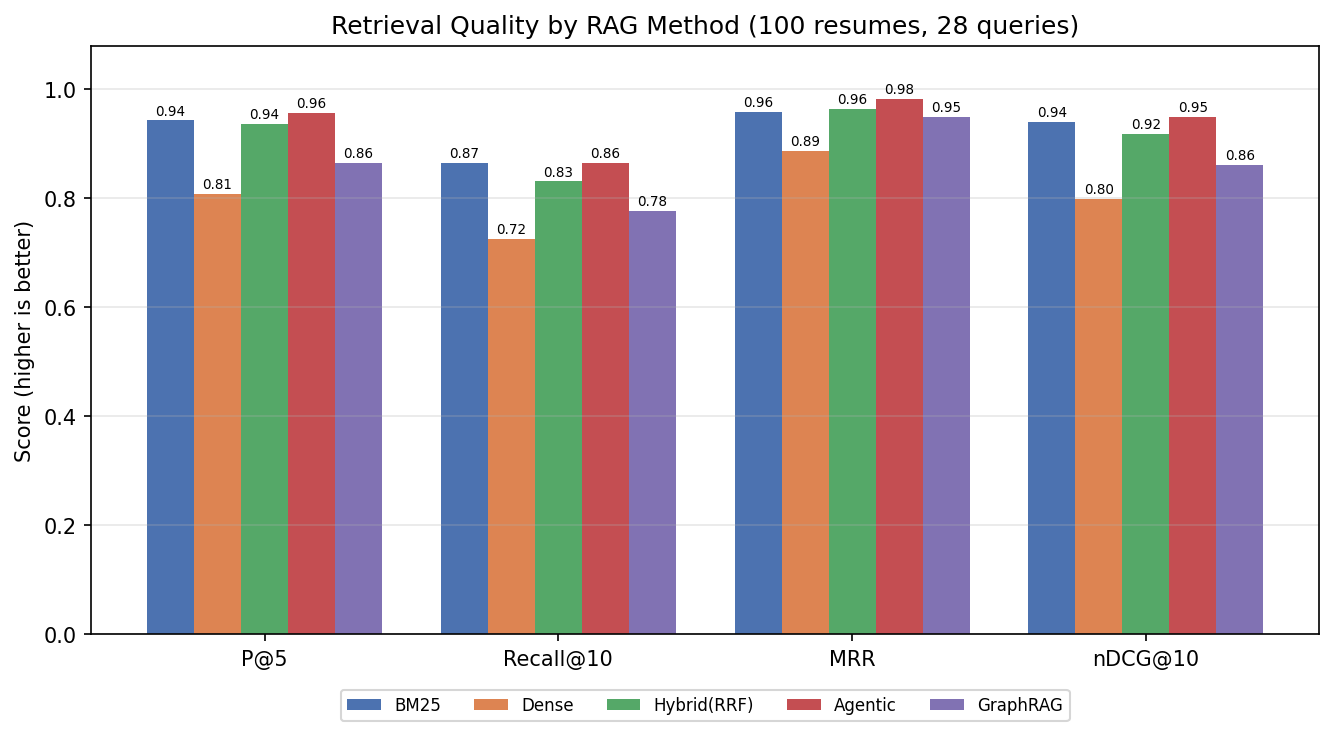
\includegraphics[width=0.92\textwidth]{figures/fig_quality_bars.png}
\caption{各方案在 P@5 / Recall@10 / MRR / nDCG@10 上的对比。}
\label{fig:quality}
\end{figure}

\subsection{时延与成本}
图~\ref{fig:latency} 为中位单查询时延（对数轴），图~\ref{fig:tradeoff} 为「质量–时延」权衡。
\textbf{Agentic 的 5.4\,秒/查询}来自 2 次真实 LLM 往返；\textbf{GraphRAG 查询期仅 30\,ms}，因为其 LLM 成本\textbf{前置在建图阶段}
（100 次抽取、20.4\,s、\$0.034）。全流程 LLM 共 156 次、提示 token 16.4 万、补全 token 1.5 万，\textbf{总成本 \$0.06}。

\begin{figure}[H]
\centering
\begin{minipage}{0.49\textwidth}
\centering
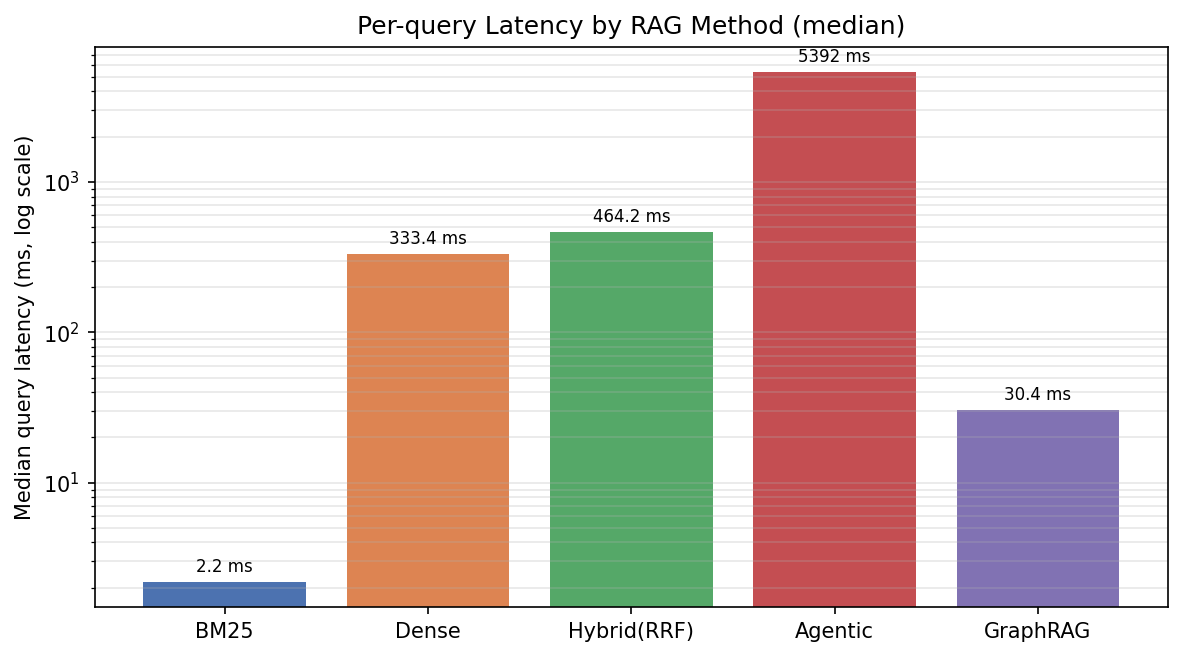
\includegraphics[width=\textwidth]{figures/fig_latency_bars.png}
\end{minipage}\hfill
\begin{minipage}{0.49\textwidth}
\centering
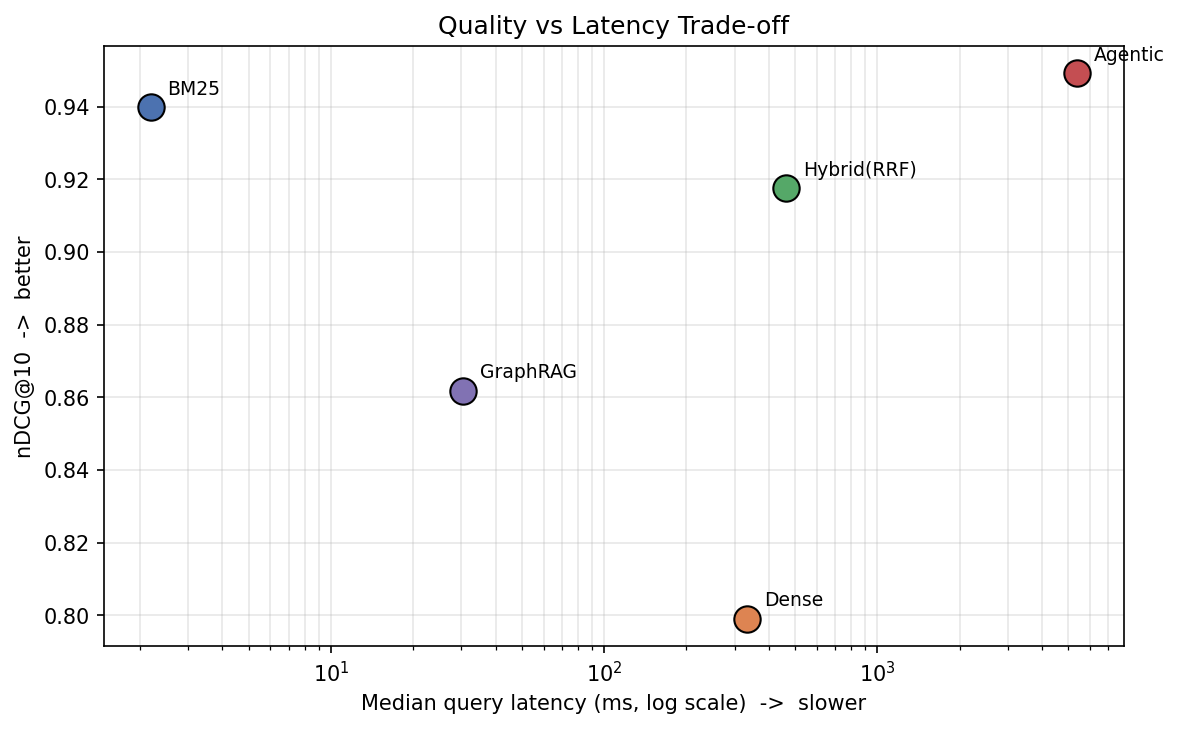
\includegraphics[width=\textwidth]{figures/fig_tradeoff.png}
\end{minipage}
\caption{左：中位单查询时延（对数轴）。右：nDCG@10 与时延权衡——\textbf{BM25 位于左上「帕累托甜点」}（高质量、最低时延），Agentic 在右上（最高质量、约 2000$\times$ 时延）。}
\label{fig:latency}
\label{fig:tradeoff}
\end{figure}

\subsection{逐查询分析}
图~\ref{fig:heatmap} 为「查询 $\times$ 方法」的 nDCG@10 热力图。整体偏绿（多数查询各方法都做得好），
但有几处暴露了方法差异（见表~\ref{tab:perquery}）。

\begin{figure}[H]
\centering
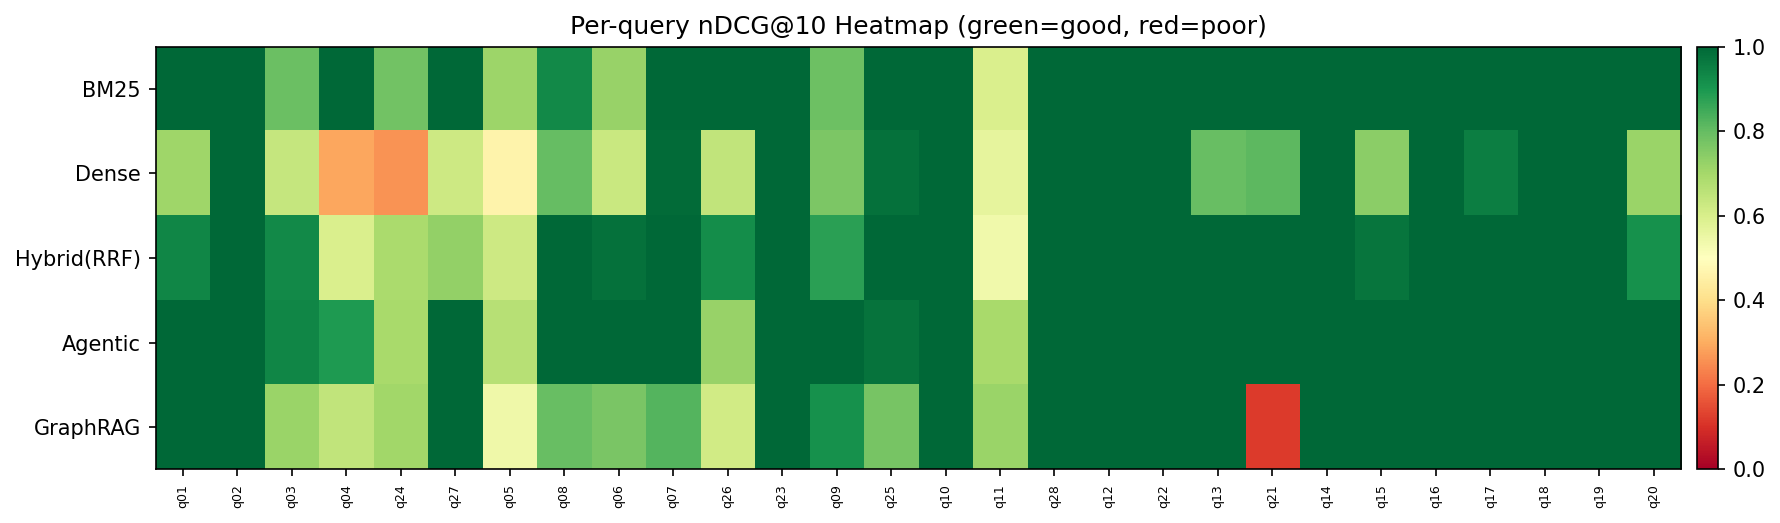
\includegraphics[width=\textwidth]{figures/fig_heatmap.png}
\caption{逐查询 nDCG@10 热力图（绿=好，红=差）。Dense 在后端/应届簇（q04、q24、q27）偏黄；GraphRAG 在 q21 出现红格。}
\label{fig:heatmap}
\end{figure}

\begin{table}[H]
\centering
\caption{代表性查询的 nDCG@10（揭示方法差异）。}
\label{tab:perquery}
\small
\begin{tabular}{llccccc}
\toprule
查询 & 说明 & BM25 & Dense & Hybrid & Agentic & GraphRAG \\
\midrule
q04 & 应届后端（中文、语义弱关键词） & \best{1.00} & 0.29 & 0.59 & 0.89 & 0.64 \\
q06 & 大模型应用（与 AI~Agent 簇歧义） & 0.72 & 0.63 & 0.98 & \best{1.00} & 0.77 \\
q21 & 运维/可观测性（术语跨簇共享） & \best{1.00} & 0.81 & \best{1.00} & \best{1.00} & 0.12 \\
q24 & 资深后端（“分布式/微服务”语义） & \best{0.78} & 0.26 & 0.69 & 0.69 & 0.71 \\
q23 & 向量检索（簇词高度可分） & 1.00 & 1.00 & 1.00 & 1.00 & 1.00 \\
\bottomrule
\end{tabular}
\end{table}

\subsection{关键发现}
\label{sec:findings}
\begin{enumerate}
\item \textbf{为什么 BM25 这么强？} 本简历语料\textbf{技能术语密集且中英混排}（中文简历也写 \texttt{Spring Boot/Kafka/Redis}）。
      检索意图与岗位簇高度由\textbf{离散技能词}决定，正是 BM25 的主场；语义改写收益空间小。
\item \textbf{Dense 为什么弱？} \texttt{all-MiniLM-L6-v2} 是\textbf{英文中心}模型。实测「high concurrency backend Kafka」与其中文版
      余弦仅 \textbf{0.10}，却与无关英文短语「React frontend」高达 0.27——它\textbf{基本读不懂中文}。
      故 Dense 在中文后端/应届簇（q04=0.29、q24=0.26）大幅失分。
\item \textbf{Agentic 在哪里真正有用？} 在\textbf{语义/歧义}查询上：q06（大模型应用 vs AI~Agent 簇共享 “RAG”）BM25 仅 0.72，
      Hybrid/Agentic 升到 0.98/1.00；q04 经 LLM 重排从 Dense 的 0.29 救回到 0.89。但代价是 2 次 LLM 往返。
\item \textbf{GraphRAG 为什么会崩？} 二值技能图\textbf{丢失词频与上下文}：q21「可观测性」中，许多后端简历正文也提
      Prometheus/Grafana，被抽成同名技能节点，与 SRE 候选人\textbf{无法区分}，导致 nDCG 跌到 0.12；
      而 BM25/Hybrid 用全文词频把真正的 SRE 排在前面。
\item \textbf{基准自身的局限（诚实声明）}：ground truth 基于技能标签，与 GraphRAG 的技能抽象\textbf{同处一个语义空间}，
      理论上对 GraphRAG 有利；即便如此 GraphRAG 仍不占优，进一步说明其在本场景收益有限。
      此外 q21 暴露了\textbf{标签粒度}问题（“Observability” 标签只给了 SRE，但后端正文也含监控栈）。
\end{enumerate}

% ============================================================
\section{结论与建议}
\label{sec:conclusion}

\begin{enumerate}
\item \textbf{本简历集上谁更优？} 论\textbf{绝对质量}是 Agentic；论\textbf{工程性价比}是 \best{BM25}：
      它以可忽略的质量差距换取 $\sim$2000$\times$ 时延优势与零成本，位于质量–时延帕累托前沿的甜点。
\item \textbf{各形态适用场景}：
   \begin{itemize}
   \item \textbf{BM25}：术语密集、对延迟/成本敏感、以关键词为主的检索（如本简历/JD 匹配的快路）。
   \item \textbf{Dense}：跨语言/同义改写/口语化查询；但\textbf{必须换多语言或中文向量模型}（如 bge-m3、multilingual-e5），
         本英文 MiniLM 不适合中文语料。
   \item \textbf{Hybrid(RRF)}：兼顾精确与语义、且想要稳健 MRR 的\textbf{生产默认}；需控制稠密路噪声。
   \item \textbf{Agentic}：高价值、低 QPS、对 Top-1/Top-3 质量极敏感的场景（精排/复核）；按需触发。
   \item \textbf{GraphRAG}：需要\textbf{多跳关系推理}（“同时做过 A 又主导过 B 的人”）的查询；
         单纯「按技能找人」用它\textbf{得不偿失}。
   \end{itemize}
\item \textbf{本项目当前是哪种形态？} 经代码核对（\texttt{ResumeRagService} / \texttt{HybridRagService} / \texttt{InternalWorkflowController}）：
      本项目是 \best{Hybrid RAG + Agentic 重排}——Milvus 稠密向量检索 + 词法(BM25-like)检索，
      按 \textbf{RRF 加权融合}（\texttt{fuseRRFWeighted}），并叠加 \texttt{agentic\_overlap\_rerank}（usefulnessScore/selectedChunks）；
      chunk 粒度 recursive(500,100)，相似度阈值 0.35。即对应本基准的 \textbf{(c)+(d)} 组合。
      （注：仓库 \texttt{application.yml} 默认嵌入模型为 \texttt{text-embedding-3-small}；本离线基准按任务用本地 \texttt{all-MiniLM-L6-v2} 以保证可复现。）
\item \textbf{GraphRAG 真的解决问题了吗？} \textbf{在本场景没有}。它查询期快、可解释，但二值技能图丢信息，
      整体 nDCG（0.862）低于 Hybrid（0.918）与 BM25（0.940），且在术语共享查询上崩塌。
      它的价值在\textbf{关系/多跳}而非「技能召回」。本项目保留图能力（\texttt{ResumeGraphService}/Neo4j）用于关系分析是合理的，
      但\textbf{不应让 GraphRAG 取代 hybrid 主检索路}。
\item \textbf{局限性}：(i) 100 份、单标注者规则型 GT，规模有限；(ii) GT 为技能标签二值相关，未做人工分级；
      (iii) Dense 用英文 MiniLM，是\textbf{下界}而非稠密上限；(iv) Agentic/GraphRAG 受 LLM 抽取/重排稳定性影响。
\end{enumerate}

% ============================================================
\section{面试问答（基于本评测的实测口径）}
\label{sec:qa}
\begin{description}[style=nextline,itemsep=7pt,leftmargin=1.2em]
\item[Q1：你的 RAG 是什么形态？]
   Milvus 稠密向量 + 词法 BM25 的\textbf{混合检索}，用 \textbf{RRF} 融合，再加一层\textbf{ agentic 重排}；
   chunk 级（500/100 重叠）召回，阈值 0.35。即「Hybrid + Agentic rerank」。
\item[Q2：准确率/召回率多少？]
   在自建 100 简历 / 28 查询基准上：生产同构形态（Hybrid）\textbf{P@5=0.936、Recall@10=0.831、nDCG@10=0.918、MRR=0.964}；
   叠加 agentic 重排后升至 \textbf{P@5=0.957、nDCG@10=0.949、MRR=0.982}。纯 BM25 基线 nDCG@10=0.940。
\item[Q3：怎么监控？]
   线上以 Prometheus/Grafana 采集：检索时延、Milvus 命中数/相似度分、空召回率、低于阈值占比、
   rerank usefulnessScore、LLM 调用数/token/成本；离线则用本 harness 的 P@5/Recall@10/MRR/nDCG@10 做\textbf{回归基准}，
   每次改动重算并对比 \texttt{metrics.json}。
\item[Q4：GraphRAG 相比 Hybrid 的增益与代价？]
   \textbf{增益}：查询期极快（30\,ms vs 464\,ms）、可解释、天然支持多跳关系问题。
   \textbf{代价}：建图需 100 次 LLM 抽取（\$0.034、20\,s）、二值图丢词频/上下文，
   本场景质量反而更低（nDCG 0.862 vs 0.918），术语共享查询会崩（q21=0.12）。
   结论：\textbf{按技能找人用 Hybrid；多跳关系推理才上 GraphRAG}。
\end{description}

% ============================================================
\section{复现与降级说明}
\label{sec:repro}
\subsection{一键复现}
\begin{verbatim}
cd reports/rag_comparison/harness
python corpus.py          # 抽取 100 简历 -> cache/corpus.json
python ground_truth.py    # 生成 queries.json + ground_truth.json
python run_eval.py        # 跑 5 方案 -> metrics.json / runs.json（LLM 结果缓存）
python make_plots.py      # 生成 figures/*.png
\end{verbatim}
产物：\texttt{metrics.json}（原始指标）、\texttt{ground\_truth.json}、\texttt{queries.json}、\texttt{runs.json}（逐查询明细）、
\texttt{graph\_cache.json}（GraphRAG 实体缓存）、\texttt{figures/}（图表）。

\subsection{环境与真实性}
Python 3.8.10；依赖：\texttt{rank\_bm25, sentence-transformers~3.0.1, torch~2.4.1, networkx, scikit-learn,
matplotlib, PyMuPDF, jieba, numpy}。LLM 为 DeepSeek \texttt{deepseek-chat}（真实调用，共 156 次，\$0.06）。
所有指标来自真实检索与真实 LLM 响应，\textbf{无编造}。

\subsection{降级点（诚实标注）}
\begin{itemize}
\item \textbf{Dense 未降级}：原计划「装不上则退化 TF-IDF」，实测 \texttt{sentence-transformers}+MiniLM \textbf{安装并运行成功}，
      Dense 为真实 MiniLM 结果（\texttt{metrics.json} 中 \texttt{dense\_degraded=false}）。
\item \textbf{网络}：本机系统代理(127.0.0.1:7999)触发 Python3.8 SSL bug，统一以直连(\texttt{NO\_PROXY=*})+清华镜像安装依赖、
      \texttt{huggingface.co} 直连下载模型——属环境适配，非指标降级。
\item \textbf{时延口径}：以\textbf{中位}时延为准；\texttt{avg\_latency\_ms} 含首查询冷启动（jieba/模型预热），故偏大，已在 \texttt{metrics.json} 一并保留。
\end{itemize}

\end{document}
